\section{Technische Ausgangssituation}
\label{sec:technische_ausgangssituation}

\begin{figure}[h]
	\begin{center}
		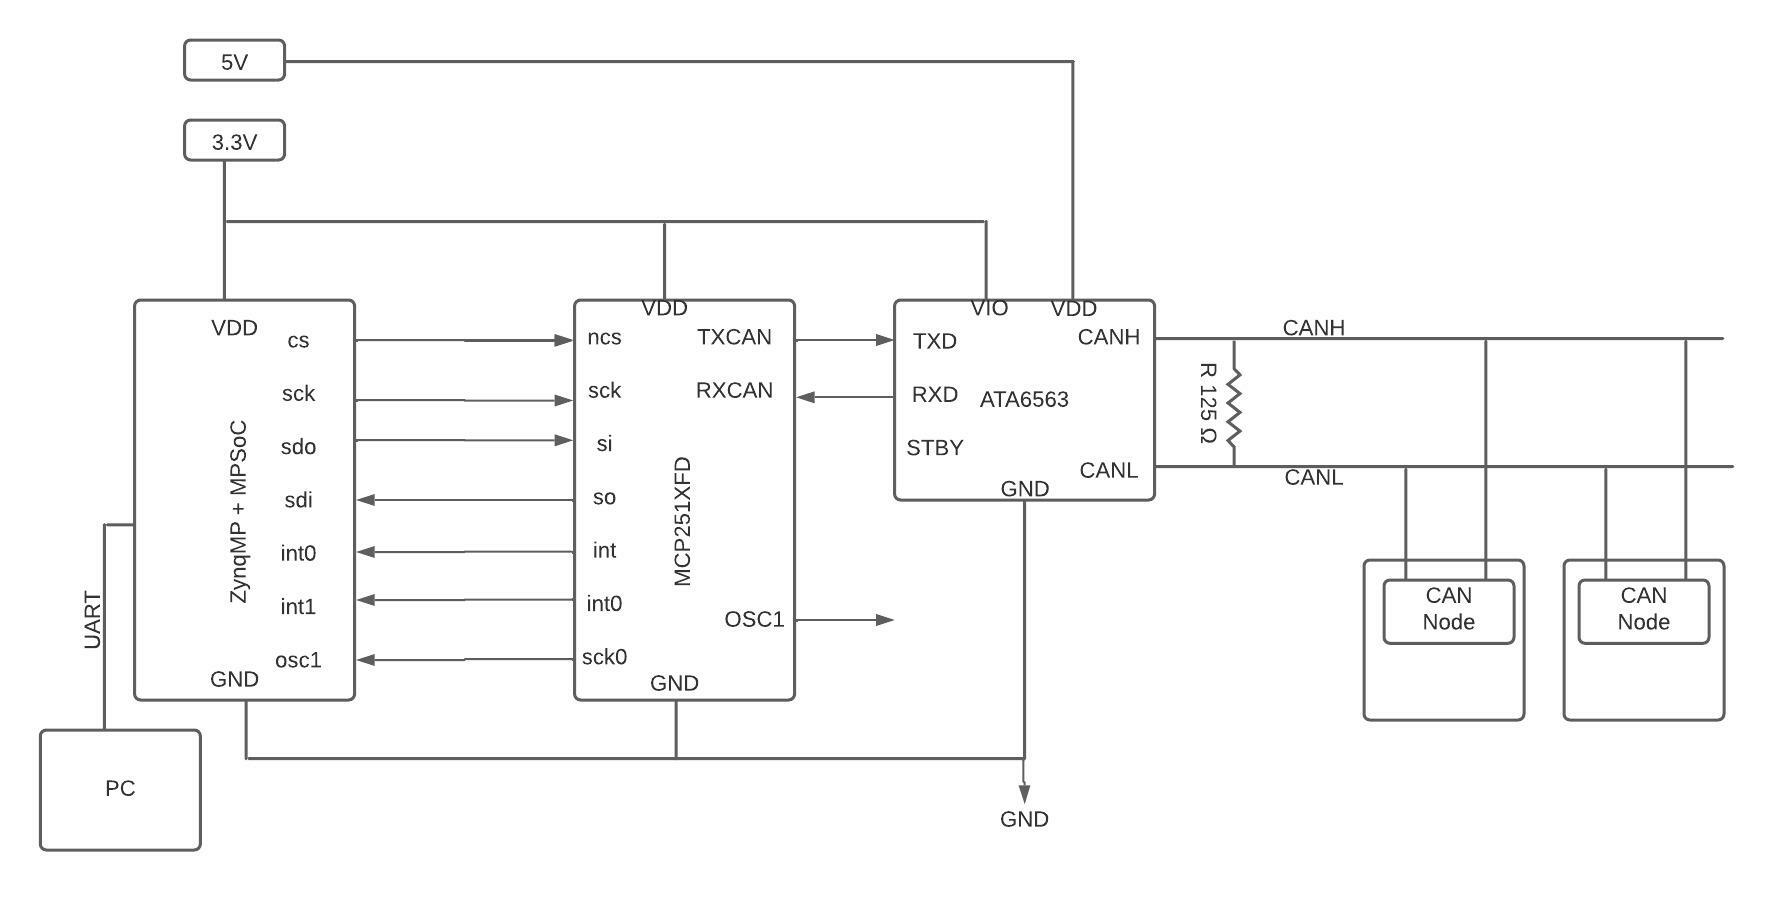
\includegraphics[width=1.2\textwidth]{./images/can_bus_system.jpeg}
	\end{center}
	\vspace{-3pt}
	\caption[CAN System Diagram]{CAN System Diagram} % Eckige Klammer (optional): Caption-Text in Abbildungsverzeichnis
	\label{fig:can_system_diagram}
	\vspace{-5pt}
\end{figure}

Das Bild auf der Abbildung \ref{fig:can_system_diagram} stellt die Verschaltung zwischen der MCP251xFD CAN Controller und der ZynqMP Plattform dar. Aufgrund der hohen Lizenzgebühren für den internen Ultrascale CAN-Bus-Controller wird ein externer CAN-Controller mit Serial Peripheral Interface (SPI) als Ersatz verwendet, um die Gesamtkosten des Systems zu reduzieren. Das SPI Interface wird also verwenden, um sowohl der CAN-Controller zu  konfigurieren, als auch die CAN-Bus-Daten bis zum FPGA zu übertragen. Auf dem Xilinx FPGA Board werden außer viele andere Peripheriegeräte auch ein SPI-Controller implementiert, mit dem Zweck, die Daten, die vom externen Peripheriegeräte kommen, zu kontrollieren. Zwischen dem MCP251XFD und dem physikalischen Zweidraht-CAN-Bus ist ein CAN-FD Transceiver (ATA6563 von Microchip) zu sehen, der als Schnittstelle zwischen beiden dient. Der bietet unterschiedlicher Empfangs- und Sendefähigkeiten mit einer Hochgeschwindigkeits von bis 5Mbit/s. In den folgenden Abschnitt gebe ich die Vorteile, ein CAN-Bus zu verwenden.